% !TEX program = xelatex
\documentclass[
  10pt,
  twoside,
  openany,
  b5paper, % 以上均为 ctexbook 提供的文类选项
  colorscheme = basic, % 请根据需要选择或定制配色方案
]{qyxf-book}
\usepackage{pdfpages}
\usepackage[contents = 钱院学辅, scale = 15, color = black, angle = 50, opacity = .10]{background}
\includepdfset{pagecommand={\thispagestyle{plain}}}

\title{算法设计与分析实验报告}
\subtitle{Lab Reports of Analysis and Design of Algorithms}  % 可选
\author{计算机钱81杨雨龙}
\date{2021 年 2 月 3 日}
%\typo{AlphaGo}  % 排版人员信息,选填

% 定制元信息
\org{\Large\textit{钱学森书院学业辅导中心}\\\textsc{Qian Xuesen College Academic Counseling Center}}
\footorg{\textsc{Qian Yuan Xue Fu}}
\cover{
	\begin{tikzpicture}[remember picture, overlay]
		\begin{pgfonlayer}{background}
			\node at ($(current page.east)+(0in,0in)$){
				
\includegraphics[width=.8\textwidth]{cover.png} };
		\end{pgfonlayer}
	\end{tikzpicture}
}
\license{}  % 清空许可证信息

% 调整封面标题大小
\renewcommand{\titlefont}{\Huge\bfseries}
\renewcommand{\subtitlefont}{\LARGE\itshape}

\begin{document}
\maketitle
\chapter*{前言}
\thispagestyle{empty}

本资料是计算机81~86班“算法设计与分析”专业选修课(2020年秋季学期)配套实验的参考实验报告。在该门课程中,作者凭借本报告获得了实验部分的满分,因此将拙作公开出来,供学弟学妹们批评探讨。本报告在完成之后尚未经高人阅读检验,难免会有疏漏,希望读者在参考时能够持怀疑态度,不吝指出错误之处,或者提出更好的算法。有些算法的理论分析部分在课本上已经阐述的很详细,报告中就从简处理。报告中的实验代码有的用Java,有的用C++,还有的用Python,只是语言上有所区别而已,并不影响解题思想。本课程当时推荐使用Java语言,便于直接白嫖课本上的代码。不过鉴于课本上的代码其实也不一定能跑的通,所以用什么语言看个人习惯和喜好就可以了。

“算法设计与分析”课程实验部分占总成绩20\%,实验涉及课程中分治,动态规划,贪心,搜索四个章节。贪心三题(三、四、五)选做一题,搜索一题必做一题选做(第七题)。每周做一个章节,每做完一道题验收一次,期末提交报告。验收时助教会要求学生当场解释算法原理并运行测试样例。如果遇到问题助教会帮你解决。2020秋季学期本课程是2.0学分选修课,不过据说以后会增加学分、延长课时、变成必修。关于如何在实验中取得较好成绩,作者有如下经验可供参考:
\begin{enumerate}
	\item 严格按照老师安排的计划完成实验并准时验收。当时老师要求我们一周验收一题,那最好就按照计划一周验收一题。既不要等期末的时候突击写代码,一次性验收好几个,也不要实验刚一开始就把所有实验代码都写完给助教老师验收。因为本课程选课人数较多,如果不按计划来会造成老师和助教工作上很多麻烦,给他们留下坏印象,成绩自然也会受到影响。
	
	\item 验收时尽量确保代码调试完成,起码要保证运行测试样例时非常顺利。并且验收前尽量把算法思路理顺,从复杂度分析、算法原理、数据结构、代码结构、问题的难点和解决思路等方面都理解透彻再去验收,确保验收时思路清晰不卡壳。作者当时的做法是每做完一个实验就把这次实验的报告仔细撰写出来,然后再去验收,既有利于理顺自己的思路,也方便期末整理报告。
	
	\item 完成选做题。当时实验要求是贪心三选一,搜索部分第六题必做,第七题选做。言外之意很可能是做第七题会额外加分。并且最后公布的完成情况表格中也确实把第七题单独列了出来。当时的第七题选做并不会花很多时间,原理和第六题没什么区别,甚至只需要在第六题的基础上稍微修改一下就行了。因此尝试一下肯定是有利的。

	\item 认真撰写报告。实验报告永远是形式大于内容,因为算法课这么多学生不可能挨个仔细去看你的内容。因此只要排版整洁一点、页数看上去多一点,分数就会高。这一点对所有大面积教学课程都是一样。

\end{enumerate}
\newpage
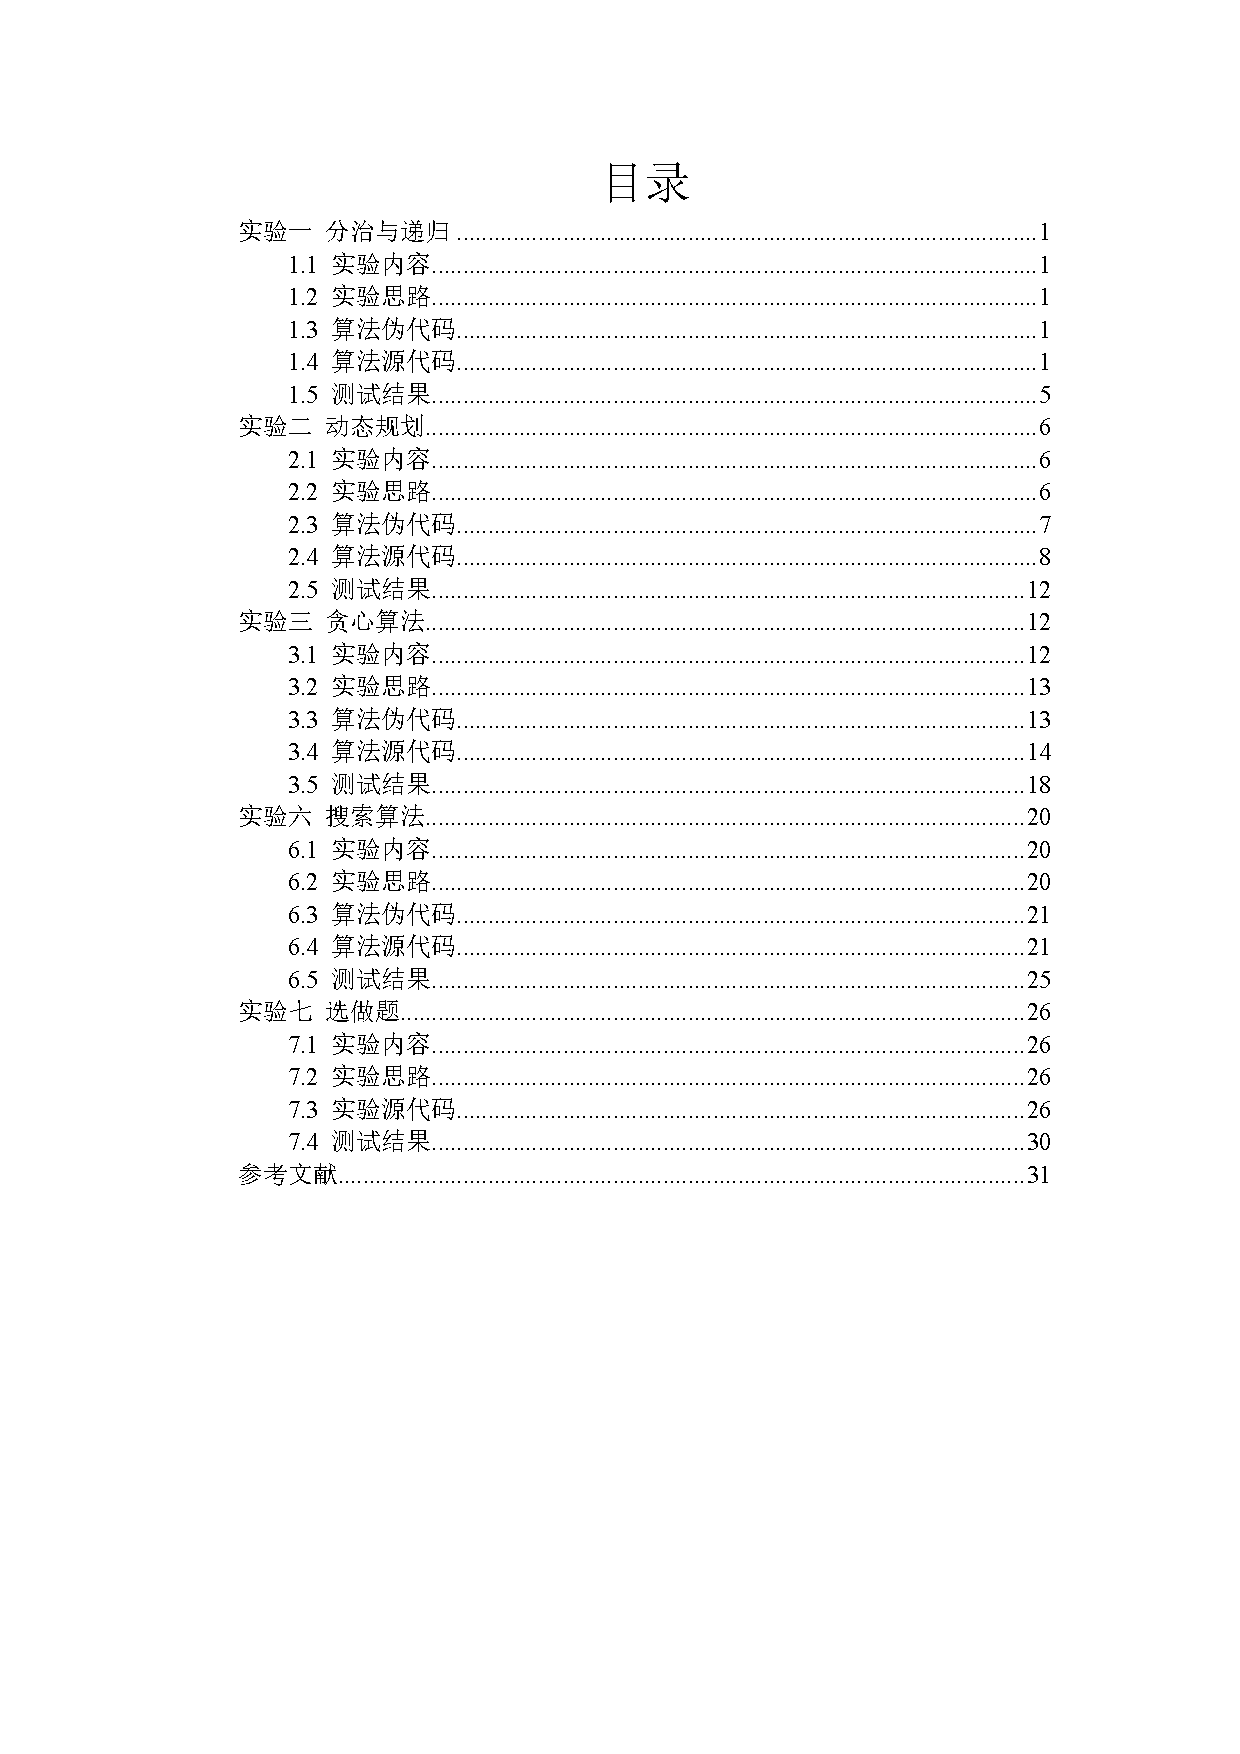
\includepdf[pagecommand = {\thispagestyle{empty}}, pages = - ]{toc.pdf}
\newpage
\setcounter{page}{1}
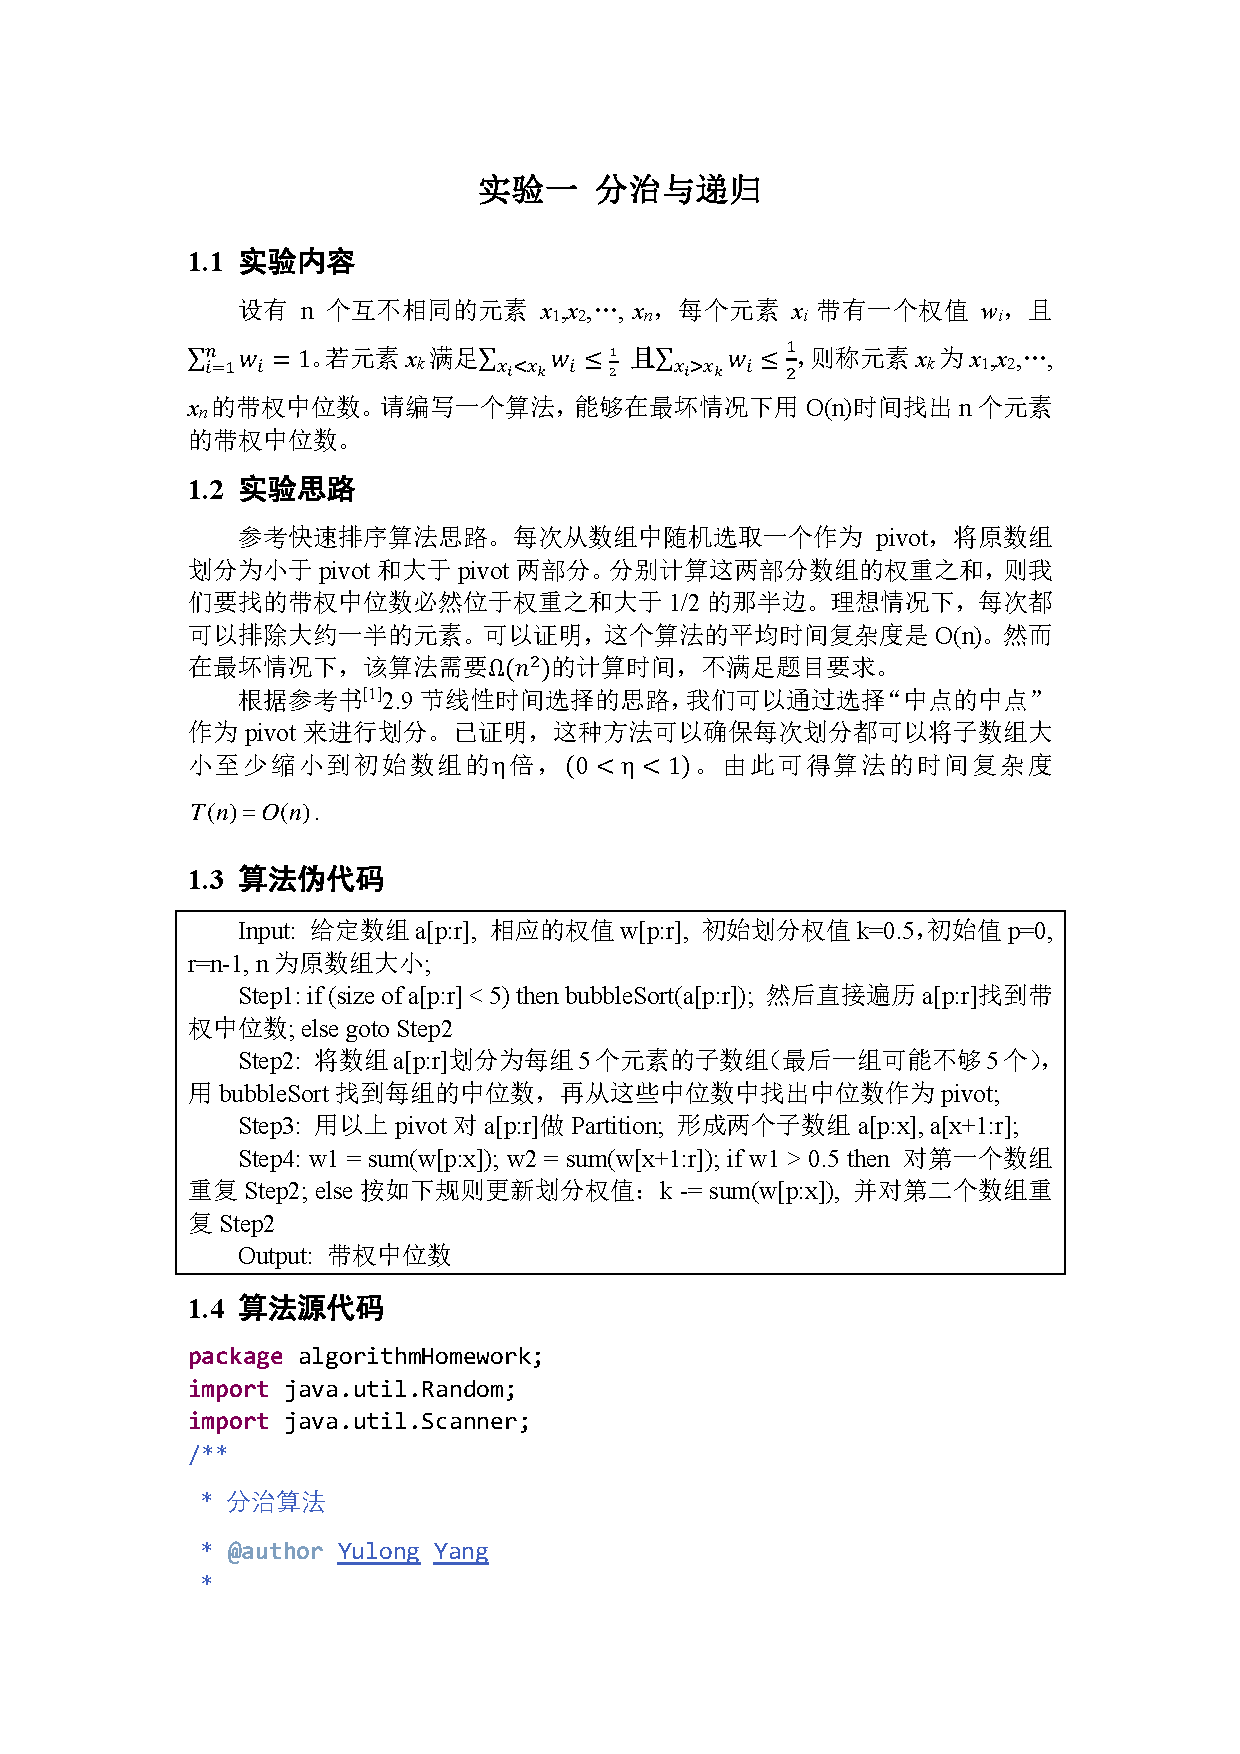
\includepdf[pages = - ]{content.pdf}

\includepdf[pagecommand = {\thispagestyle{empty}}, pages = - ]{lastpage.pdf}

\end{document}